\documentclass{article}
\usepackage{geometry}                % See geometry.pdf to learn the layout options. There are lots.
\geometry{a4paper}                   % ... or a4paper or a5paper or ... 
%\geometry{landscape}                % Activate for for rotated page geometry
%\usepackage[parfill]{parskip}    % Activate to begin paragraphs with an empty line rather than an indent
\usepackage{graphicx}
\usepackage{amssymb}
\usepackage{amsthm}
\usepackage{amsmath}
\usepackage{mathrsfs}
\usepackage[french]{babel}
\usepackage{color}
\usepackage{listings}
\definecolor{javared}{rgb}{0.6,0,0} % for strings
\definecolor{javagreen}{rgb}{0.25,0.5,0.35} % comments
\definecolor{javapurple}{rgb}{0.5,0,0.35} % keywords
\definecolor{javadocblue}{rgb}{0.25,0.35,0.75} % javadoc

\lstset{language=Java,
basicstyle=\ttfamily,
keywordstyle=\color{javapurple}\bfseries,
stringstyle=\color{javared},
commentstyle=\color{javagreen},
morecomment=[s][\color{javadocblue}]{/**}{*/},
stepnumber=2,
numbersep=10pt,
tabsize=4,
showspaces=false,
showstringspaces=false}
\usepackage[applemac]{inputenc}
\newtheorem{theorem}{Théorème}
\newtheorem*{definition}{Définition}
\newtheorem*{exercice}{Exercice}
\hyphenpenalty=10000

\title{Secure Airport Tower\\Final Report}
\author{frederic.jacobs@epfl.ch\\ hantao.zhao@epfl.ch}
\begin{document}
\maketitle 
\section{Setting up our project}
The first thing to point out is the fact that we used the JRE 1.7 because we use switches on Strings and other features of the JRE 1.7. It runs smoothy on Windows, Mac and Linux (avoid compiling with the OpenJDK).  Once you created the project in Eclipse, don't forget to add the libraries that are in \verb /src/libs  to the build path. Once that's done, you're ready to go. 

Java 1.7 SDK has some flaws on Unix-Platforms though. Written once, runs everywhere might not be true depending on the runtime. It turned out that JRE 1.7 was the most stable on Windows. 

For use of encryption with our Tower, it generates at runtime a file called \verb MyKey  that stores the key in a plane compatible format inside the main folder. 

\section{Project's Architecture}
Our program is structured into different packages. There are two classes that are executable.  \verb AirportGUI.java  launches everything needed to run the tower while \verb TestPlane.java  launches everything required for the plane to run. We are in this section going to give a quick overview of what each class does. For further information please check out our JavaDoc. 
We have some encapsulation flaws that are linked with late minute refactoring.

\newpage

\begin{figure}[!]
 \hspace{40px}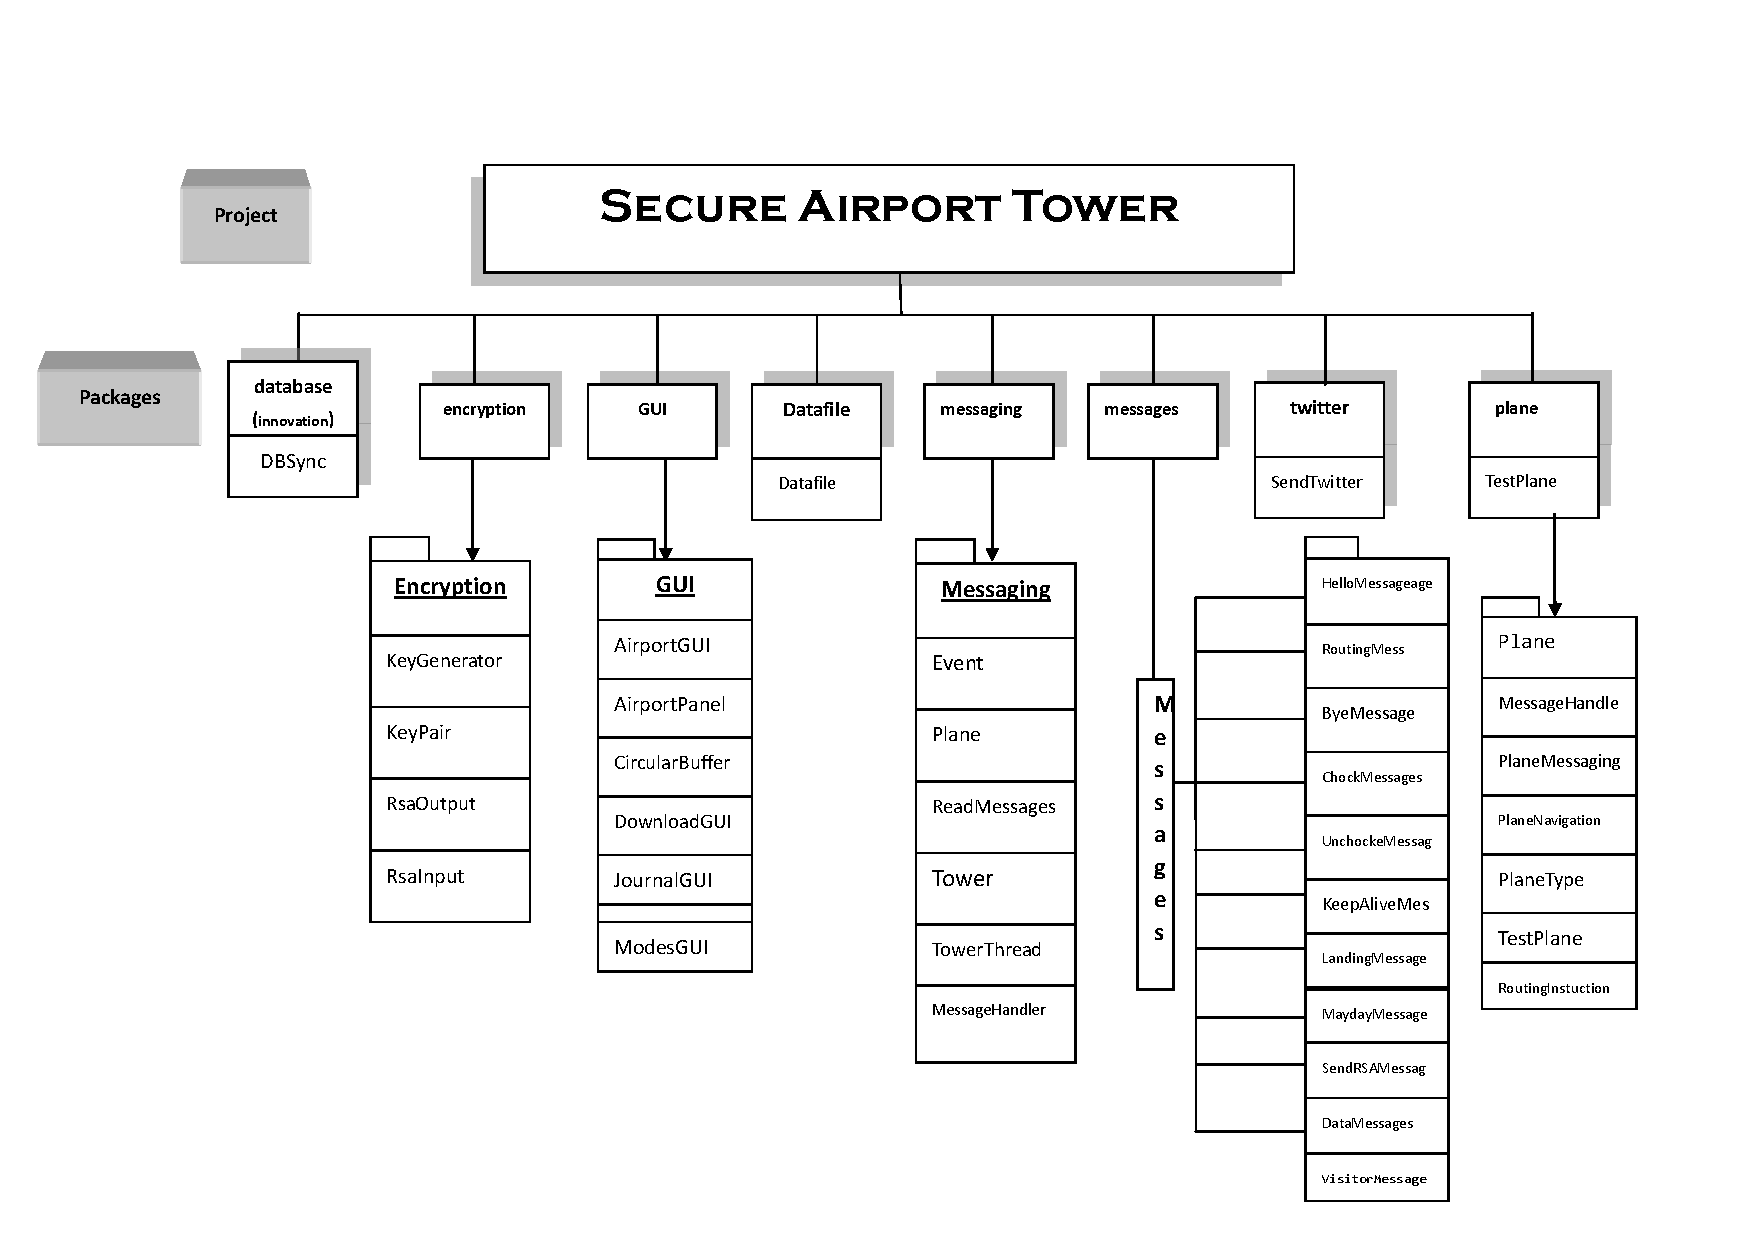
\includegraphics[width=0.8\textwidth]{UML.pdf}
 \caption{UML diagram of the project}
\end{figure}

\newpage

\subsection{Database}
This is a separate package that is specific to our innovation. We designed a REST-API that allows to fetch the logs and the position of planes. To do that, we had to have a specific syncing thread. Updating the position each time a plane sends a keep-alive wasn't sustainable so we chose to update the database every second with the latest positions. That is \verb DBSync.java  's job. It fetches the positions from the journal and updates them automatically in the Tower only if they changed. We are using a JSON format that is very friendly in JavaScript for future applications such as web apps. 

\subsection{DataFile}

\verb DataFile.java  is responsible for creating DataMessages objects from a File. It can also write a File from a bunch of DataMessages. The DataMessages should be routed to this DataFile. After some refactoring we didn't stick to the original description of the DataFile because we believed it didn't make much sense to have this bunch of superficial variable (or we may not have understood what they were doing). We managed to get this class working with a slightly modified version of the original test. 

\subsection{Encryption}
The \verb encryption  package provide all the tools required in this project related to encryption. 
\begin{enumerate}
\item \verb KeyGenerator.java  - It is responsible for generating new RSA keys, both public and private. It simply requires a given size and it will generate the keys for you.
\item \verb KeyPair.java  - Nothing more than a simple wrapper object to store RSA Keys. 
\item \verb RsaInputStream.java  - This is a tool for reading encrypted blocks of data coming from the network. It requires a KeyPair with a private key to decrypt the blocks coming from the network. 
\item \verb RsaOutputStream.java  - Exactly the opposite of the preceding class. It is designed to encrypt blocks of data and splitting them to be RSA-safe depending on the size of the size of the key. 
\end{enumerate}

\subsection{generals}
In this package we have only one but very precious tool. It's a class called  \verb XYPosition it is used all over the project and defines what coordinates are. It is a timesaver and makes the code often more readable. 

\subsection{GUI}

The \verb GUI  package is the main package of our application. It is the main thread of our application that will launch and dispatch all the rest of the tasks. We sticked to \verb AWT/SWING  for the design. Although it is not perfect, we believe it completes it's task. We also launch a bunch of other panels. Let's quickly discover all the essential classes in the GUI.

\begin{enumerate}
\item \verb AirportGUI.java is our main class. It remains very simple but launches the Tower Singleton instance that will handle all the communication with the planes. It also handles all the different panels that are launched.  
\item \verb AirportPanel.java  is the radar screen. We only made very little changes to it to allow it to work with our classes. We also improved it for having custom red airplanes in case of MayDays.  
\item \verb Choker.java  is the our custom button to simply toggle the Choke mode. It is simple and work as expected. It's a simple button that changed from red to green depending on the choke status.
\item \verb CircularBuffer.java  is a buffer used in the AirportPanel to draw the points. It was provided. No changes.
\item \verb DownloadGUI.java  is a little box that displays the downloaded files from the plane. Nothing special here.
\item \verb JournalGUI.java  is the observer of any changes in the Journal and then automatically updates the \verb GUI  version of the journal.
\item \verb ModesGUI  - This class is the GUI of the optimization modes. It uses a ButtonGroup to let the client choose from 3 types of the modes, and it can print out the total number of passages, the total number of fuel consumption and the waiting time of per passages.  It also implements the observer so that each time we receive a bye message, the corresponded information will be updated automatically.
\end{enumerate}

\subsection{Messaging}
Messaging is the biggest part of this project. 
Let's have an overview of all the classes in this package.
\begin{enumerate}
\item \verb Circle.java  - This class is the main part to arrange the landing request of the planes and also send the routing messages to different planes. It has also a method to respond the Mayday message, called the landingUrgent. The general idea of designing the routing respond is that we judge which is the closed valid route, and add the current plane to the \verb Arraylist  of the route.For example if the landing route is valid right now we will send a landing routing message directly. In this way all the planes will be well arranged. 
\item \verb Event.java  - This class is a part of the journal. Each time a message is created or send out, it will be saved as an Event. It contain the information such as message, source, destination and the time at which it is created.
\item \verb Journal.java  - This class is a journal which will record all the event happened during the communication. It will also run the planeHasCrashed or planeDidLand method to help the GUI to print out the needed information. As it is a part of the observer mode, it extends the Observable to remind the \verb JournalGUI  when a new event is saved in.
\item \verb Modes.java  - This class is the main part of the ModesGUI, it contains three kinds of Comparator to rank the ArrayList of the tower. The comparatorChronos is based on the time order of the plane so we judge it by comparing the initial time of the planes. The comparatorFuel is based on the consummation of the plane so we judge it by comparing the consummation of the planes. The comparatorTime is based on the waiting time of the plane so we judge it by comparing the passage number of the planes.
\item \verb Plane.java  - This is the class of Plane. It is responsible for create a array of the planes in the Tour to save all the information of the planes which have communicated with the Tour. It has several parameters.
\item \verb PlanePosition.java  - This class allows to have a wrapper object for an array of Planes with an associated position, crash status and landing status.
\item \verb ReadMessages.java  - This class aims at converting the DataInputStream into a new created message, by using the method read (for byte[]) and readInt.
\item \verb Tower.java represents the tour of airport, which have the function of receiving and sending Message with the planes. 
\item \verb TowerMessageHandler.java is the class file that handles received messages. This class help the Tower to handle communications with several planes, that is to say that each thread handles the connection with one plane.
\item \verb TowerThead.java  - This class help the Tower to handle communications with several planes, that is to say that each thread handles the connection with one plane.
\item \verb Visitor.java  - This class is the main part of the visitor pattern. It aims at handling different kinds of messages, such as Hello , KeepAlive and so on. Each time there is a message which needs to be handled in the tower-message handle it will call the visit() method so that the Visitor class will judge the type of different message and do different move to respond.
\end{enumerate}

Please note that we have a sub-package in which we define each different type of message. Since these are only wrappers, please refer to the JavaDoc to know more about them.

\subsection{Plane}
Plane is the package that contains all the classes related to our own plane. 
\verb TestPlane.java  is the main class. It supports random name generation for planes, initialization with launch settings and generates the key used for encryption.
Here are some other underlying classes.
\begin{enumerate}
\item \verb Plane.java  - This class is a wrapper class of what a plane can be. 
\item \verb PlaneMessageHandler.java  - Similar than the TowerMessageHandler but with other reactions. It helps the Plane to handle different type of messages and respond to them accordingly.
\item \verb PlaneMessaging.java  - It is the Thread handling the communication with the Tower.
\item \verb PlaneNavigation.java  - This class is taking care of the navigation of the plane. Of course, the main goal of this thread is to update on a regular basis the position of the plane.
\item \verb PlaneType.java  - This enum defines a few types of planes given in ITP-06 and assigns them their specifications.
\item \verb RoutingInstruction.java  - Just a wrapper class of a RoutingInstruction.
\end{enumerate}

\subsection{Tests}

All our unit tests. No need for further explanation. They all run.

\subsection{Twitter}
Simple static class to send a tweet with only a line of code using the \verb twitter4j  library. Neat !

\section{Q\&A}
\subsection {ITP-02}
In ITP-02, we were asked two questions. 
\begin{enumerate}
\item Is it a good idea to use a superclass to define Messages ?
\item Why is it an abstract class ?
\end{enumerate}
In a object-oriented universe like Java, we like to model things hierarchically. We want all possible types of messages to have a behavior or to have some instance variables therefore defining a super-class Messages makes a lot of sense. We were asked to have these instance variables in each Message Type so we implemented these in our super-class.

\begin{lstlisting}
byte[] planeID;  //The unique identifier of the plane
int length; //Length of the message
int priority; //Priority in PriorityQueue
int posx; //Positioning data 
int posy;
MessageType type; //Type of Message
\end{lstlisting}

The reason why we want this to be an abstract class is really straightforward. We defined a Message super-class because we expect messages to behave a given way but we also want these messages to have a type. All messages will inherit these attributes from the super-class but the super-class won't be instanciable to assure we call the right constructor when creating a message with a certain type. The keyword \emph{abstract} does exactly this. 

\section {GUI Critics}

\subsection{Interface analysis}

This project is aimed at building a friendly interface for the air control department of an airport. The special needs of security require the interface to be able to highlight the situations of crisis and emergency. We build an interface focused on the map so that it gives a good overview of the airfield and surroundings.  Another significant part is the journal. It is the record for all the exchanged messages and the pattern for the no-professional colleagues. By using the filter and the color identification system we make the complicated record of all communications between the tower and the plane in a clear and structured way.
On the other hand we must build a reliable platform for operators. We made the huge simple button to toggle the Choke/Unchoke so the operator is able to deal with crisis immediately. And everyone likes big red buttons. As required we also use the button group for the optimization routing modes. The GUI is composed of several panels. This Photoshop like design is modulable and great on multi-displays setups because you can split the interface between two screens which is pretty cool for a control center. On the other side, there is no Unity mode to join the panel together and at launch they look very messy by superposing other panels. We focused more on the back end like the syncing with the database. So our application doesn't have a neat UX which is pretty difficult to implement using AWT/Swing.

\subsection{Improvement proposal}

Our time being limited we hadn't much time to improve significally the user interface. Zooming in and out would be great to have an extended operation field for large scale routing. Another very interesting improvement would be to add an extra dimension, the altitude. Unfortunately to implement 3D we need an altitude that is more difficult to deal with because it also requires back-end modifications. Since the complicity of the project is limited to the freshmen of the computer science, the altitude of the planes wasn't taken into consideration.
Ideally we should provide for each platform a more native user-experience by sticking to the User Interface Guidelines of the given platform but since Java is cross-platform we can't really optimize that.
For instance, you could badge the dock on the Mac with the number of planes in the air. While on Windows the separate panels could be displayed using a Metro-style layout. A lot of enhancements are possible but our time too limited to implement those.

Being able to click the plane and having some advanced information like the fuel level would be really great. We would also greatly benefit from having a GUI for the planes allowing to launch them easier with custom settings.

\end{document}
